\documentclass[letterpaper,12pt,fleqn]{article}
\usepackage{matharticle}
\usepackage{tikz}
\renewcommand{\l}{\lambda}
\pagestyle{plain}
\begin{document}

\begin{center}
  \large
  Math-71 Sections 9, 11, 12

  \Large
  Homework \#11

  \large
  \textbf{Due: 5/9/2019 5:45pm}
\end{center}

\subsection*{Reading}

Read sections 11.1-11.4

\subsection*{Problem}

You work for the county tax collector's office.  You prepare a platmap that shows six lakefront properties in your
county as follows:

\bigskip

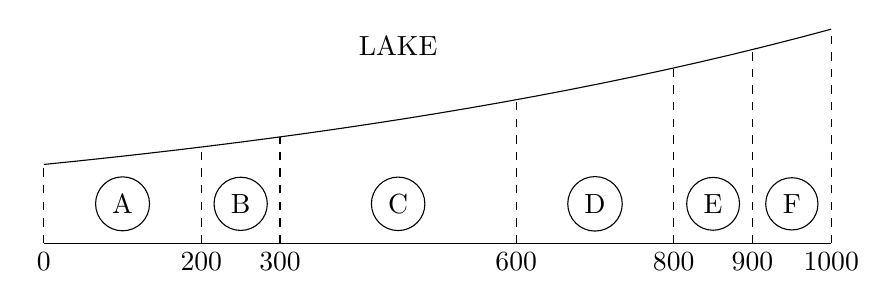
\begin{tikzpicture}
  \draw (0,0) -- (10,0);
  \draw [domain=0:10] plot ({\x},{exp(0.1*\x)});
  \pgfmathsetmacro{\a}{exp(0.2)};
  \pgfmathsetmacro{\b}{exp(0.3)};
  \pgfmathsetmacro{\c}{exp(0.6)};
  \pgfmathsetmacro{\d}{exp(0.8)};
  \pgfmathsetmacro{\e}{exp(0.9)};
  \pgfmathsetmacro{\f}{exp(1)};
  \draw [dashed] (0,0) -- (0,1);
  \draw [dashed] (2,0) -- (2,\a);
  \draw [dashed] (3,0) -- (3,\b);
  \draw [dashed] (6,0) -- (6,\c);
  \draw [dashed] (8,0) -- (8,\d);
  \draw [dashed] (9,0) -- (9,\e);
  \draw [dashed] (10,0) -- (10,\f);
  \node [below] at (0,0) {0};
  \node [below] at (2,0) {200};
  \node [below] at (3,0) {300};
  \node [below] at (6,0) {600};
  \node [below] at (8,0) {800};
  \node [below] at (9,0) {900};
  \node [below] at (10,0) {1000};
  \node [draw,circle] at (1,0.5) {A};
  \node [draw,circle] at (2.5,0.5) {B};
  \node [draw,circle] at (4.5,0.5) {C};
  \node [draw,circle] at (7,0.5) {D};
  \node [draw,circle] at (8.5,0.5) {E};
  \node [draw,circle] at (9.5,0.5) {F};
  \node at (4.5,2.5) {LAKE};
\end{tikzpicture}

\bigskip

where the bottom boundary scale is in feet.  The lakeshore follows the equation:
\[y=e^{\frac{x}{200}}\]
for \(x\) and \(y\) in feet.

The property tax assessment for these properties is to be \$2 per square foot.

What is the property tax assessment for property C?

\end{document}
